\chapter{Context Discovery Framework}

In this chapter, we shall look at the the CueNet framework and its components: a \textit{data integration module} to model and query the various data sources and sensors, a \textit{discovery algorithm} to construct queries agnostic to what to the sources themselves, a \textit{knowledge representation module} to store relationships about the various real world objects, and finally how these parts integrate with a \textit{face verification algorithm}, which predicts if a person is present in a photo or not.

\section{Pruning Search Spaces with CueNet}

Automatic media annotation algorithms essentially assign one or more labels from a search space to a given input image. Figure \ref{fig:with-without-cuenet} shows the various approaches of constructing such a search space for such an algorithm. The traditional approach is shown in \ref{fig:with-without-cuenet}(a). These spaces were limited to a set of labels chosen by an expert, with no way of pruning the search space in case it got very large. The focus was instead on extracting the best features from images, to obtain high overall classification accuracy\cite{turk1991eigenfaces}.

\begin{figure}[t]
\centering
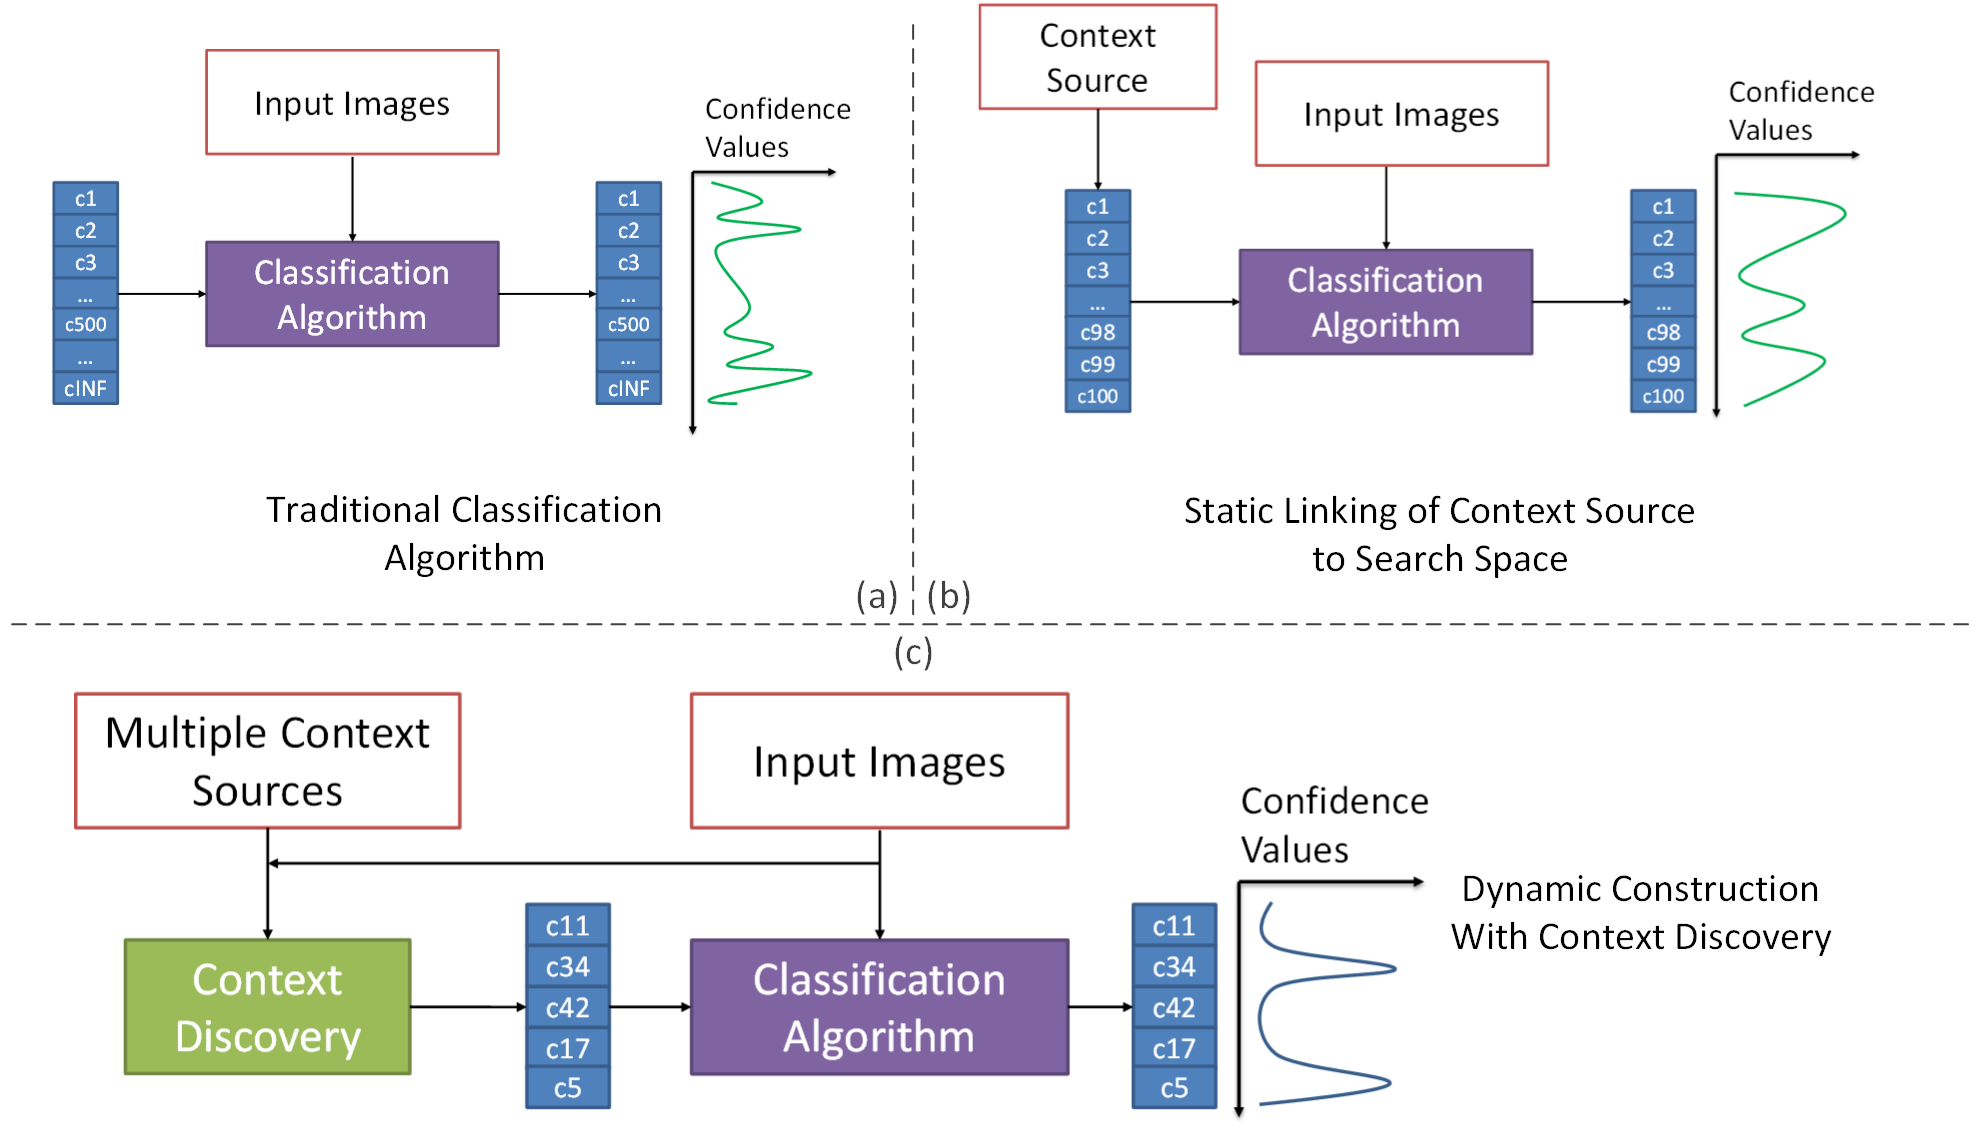
\includegraphics[width=0.95\textwidth]{media/with-without-cuenet-2.png}
\caption{The different approaches in search space construction for a multimedia annotation problem. A traditional classifier setup is shown in (a) where the search space candidates are manually specified. Context is used to generate large static search spaces in (b). The desired framework is shown in (c), which aims to produce small search spaces with many correct annotations.}
\label{fig:with-without-cuenet}
\end{figure}

With the popularity of global social networks and proliferation of mobile phones, information about people, their social connections and day-to-day activities are becoming available at a very large scale. The web provides an open platform for documenting many real world events like conferences, weather events and sports games. With such context sources, the search space construction is being delegated to one or a few sources \cite{henter2012tag, li2012fusing, naaman2005identity, o2009context,  stone2008autotagging} (figure \ref{fig:with-without-cuenet}(b)). These approaches rely on a single \textit{type} of context. For example, time and location information or social network information from Facebook to solve the face recognition problem. We refer to such a direct dependency between the search space and a data source as \textbf{static linking}. Although these systems are meritorious in their own right, they suffer from the following drawbacks: they do not employ multiple sources, and therefore the \textbf{relations} between them. By realizing that these sources are interconnected in their own way, we are able to treat the entire source topology as a network. Our intuition in this work is to navigate this network to progressively discover the search space for a given media annotation problem. Figure \ref{fig:with-without-cuenet}(c) shows how context discovery can provide substantially smaller search spaces for a set of images, which contain a large number of correct tags. A small search space with large number of true positives provides the ideal ground for a classification algorithm to exhibit superior performance.

\textbf{The CueNet framework}, provides access to multiple data sources containing event, social, and geographical information through a unified query interface to extract information from them. CueNet encapsulates our \textbf{Context Discovery Algorithm}, which utilizes the query interface to discover the most relevant search space for a media annotation problem. To ensure a hands-on discussion, we show the use of context discovery in a real world application: face tagging in personal photos. As a case study, we will attempt to tag photos taken at conference events by different users. These photos could contain friends, colleagues, speakers giving very interesting talks, or newly found acquaintances (who are not yet connected to the user through any social network). This makes the conference photos particularly interesting because no single source can provide all the necessary information. It emphasizes the need to utilize multiple sources in a meaningful way.

\begin{figure}[t]
\centering
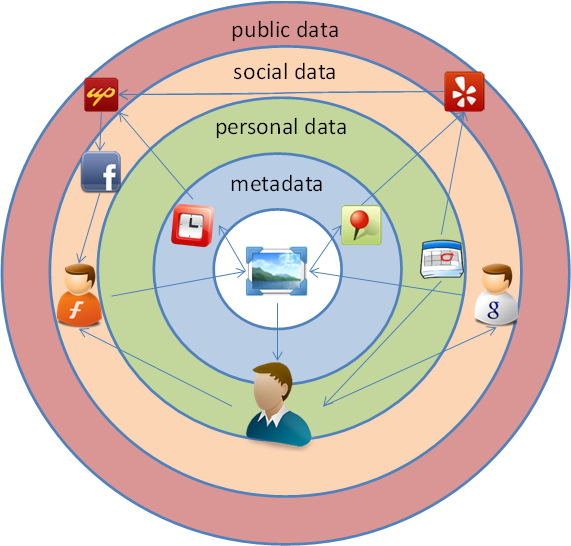
\includegraphics[width=0.65\textwidth]{media/prog-discovery.png}
\caption{Navigation of a discovery algorithm between various data sources.}
\label{fig:prog-discovery}
\end{figure}

Here is an \textbf{example} to illustrate CueNet's discovery process. Let's suppose that Joe takes a photo with a camera that records time and GPS in the photo's EXIF header. Additionally, Joe has two friends. One with whom he interacts on Google+, and the other using Facebook. The framework checks if either of them have any interesting event information pertaining to this time and location. We find that the friend on Google+ left a calendar entry describing an event (a title, time interval and name of the place). The entry also marks Joe as a participant. In order to determine the category of the place, the framework uses Yelp.com with the name and GPS location to find whether it is a restaurant, sports stadium or an apartment complex. If the location of the event was a sports stadium, it navigates to upcoming.com to check what event was occurring here at this time. If a football game or a music concert was taking place at the stadium, we look at Facebook to see if the friend ``Likes" the sports team or music band. By traversing the different data sources in this fashion, the number of people, who could potentially appear in Joe's photograph, was incrementally built up, rather than simply reverting to everyone on his social network or people who could be in the area where the photograph was taken. We refer to such navigation between different data sources to identify relevant contextual information as \textbf{progressive discovery}. The salient feature of CueNet is to be able to progressively discover events, and their associated properties, from the different data sources and relate them to the photo capture event. We argue that given this structure and relations between the various events, CueNet can make assertions about the presence of a person in the photograph. Once candidates have been identified by CueNet, they are passed to the face tagging algorithm (as in \cite{facever_pami2010}), which can perform very well as their search space is limited to two candidates.

Figure \ref{fig:cuenet-arch} shows the different components of the CueNet framework. The Ontological \textbf{Event Models} specify various event and entity classes, and the different relations between them. These declared types are used to define the \textbf{Data Sources} which provides access to different types of contextual data. The \textbf{Person Verification Tools} consist of a database of people, their profile information and photos containing these people. When this module is presented with a candidate and the input photograph, it compares the features extracted from the candidate's photos and the input photo to find the confidence threshold. In this section, we describe each module, and how the context discovery algorithm utilizes them to accomplish its task.

\begin{figure}[t]
\centering
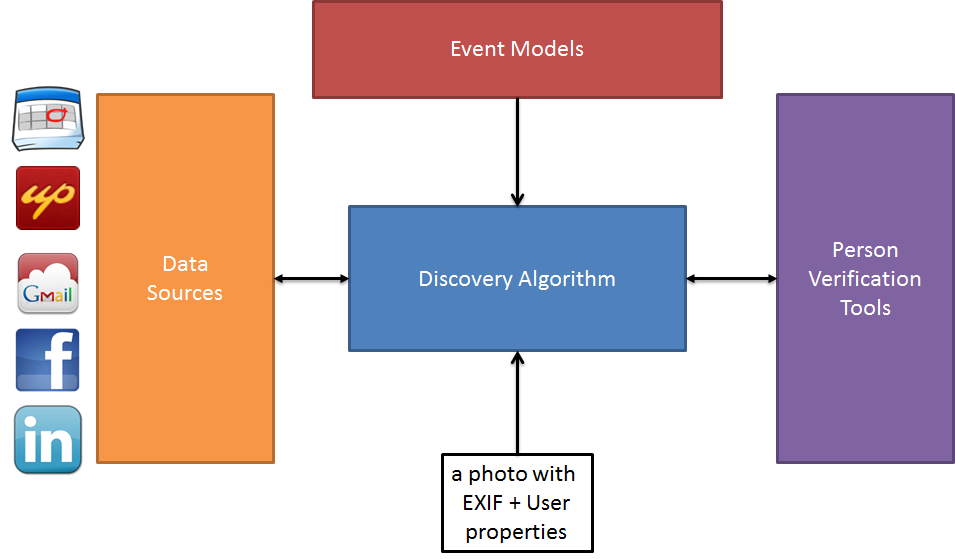
\includegraphics[width=0.9\textwidth]{media/cuenet-high-level-arch.png}
\caption{The Conceptual Architecture of CueNet.}
\label{fig:cuenet-arch}
\end{figure}

\section{General Approach}
Figure \ref{fig:cuenet-arch} shows a high level architecture of CueNet. The major functional blocks consist of a data integration system (left), which provides a uniform query interface to a multitude of autonomous data sources, which may reside within an enterprise or on the World-Wide Web \cite{halevy2001answering}; a specification of model describing real-world knowledge in terms of objects and their relations, along with any axioms and constraints to be imposed on instance graphs (top); since we are assisting face tagging application, the final block (right) consists of a set of hooks to invoke appropriate face tagging algorithms by providing a set of candidate for the input photo. In this work, we shall assume verification semantics in such a tagging algorithm, where given an input photo and a candidate person, the algorithm returns true or false (with a confidence score). Face recognition models would have to be retrained when the candidate set changes. Also, as described in chapter 3, the state-of-the-art techniques for face verification perform much more reliably than their recognition counterparts. At the heart of CueNet, lies the context discovery algorithm. Given a photo the algorithm constructs a context network with all the known information. Using the knowlege base, the algorithm constructs queries to be executed on the interface provided by the data integration layer. Objects which are returned are merged into existing context network. New entities in the network are passed to the face tagging algorithm to check for their presence in the photo. If they are present, the context network is altered to reflect this fact. The execute-merge cycle is iteratively performed until all the faces are tagged, or the data integration module is unable to furnish any new data.

\section{Execution Trace}
In this section, we will trace the execution on two different photos, to see how the different modules interact to produce context networks, and how they are used to tag faces. The first example will be a relatively simpler one, requiring only 2 data sources, whereas the second photo will require multiple sources to sucessfully tag all photos.

\subsection{Simple Case}

Consider the photo shown in figure \ref{fig:stacktrace-simple-torsten-hidden}. For the purposes of this trace, we assume that we have access to the sources shown in figure \ref{fig:stacktrace-simple-sources} through the data integration module. Given, an input photo, the knowledge base is queried to find what other objects can be associated with an photo object. The KB stores the information that every photo consists of an EXIF header, which stores timestamp and location coordinates and a fact which states that every photo is owned by a user object, where \textbf{owner-of} is a relationship described in the KB. This knowledge is used to construct the context network shown in figure \ref{fig:exif-network}.

\begin{figure}[ht]
\begin{minipage}[b]{0.45\linewidth}
\centering
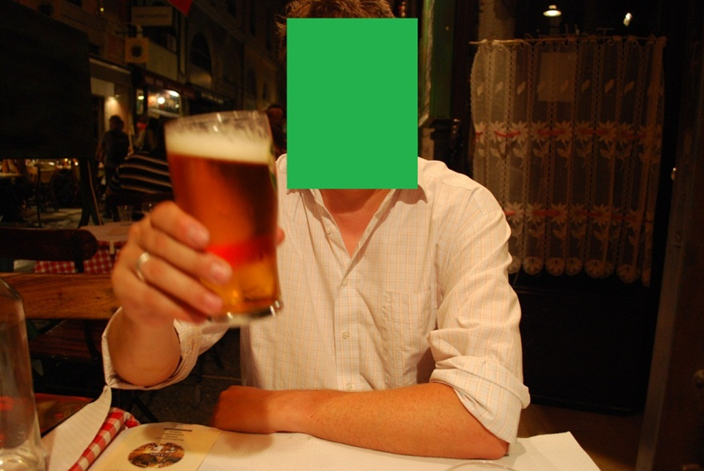
\includegraphics[width=\textwidth]{media/chapter4/stacktrace/torsten-hidden.png}
\caption{Input Photo.}
\label{fig:stacktrace-simple-torsten-hidden}
\end{minipage}
\hspace{0.5cm}
\begin{minipage}[b]{0.45\linewidth}
\centering
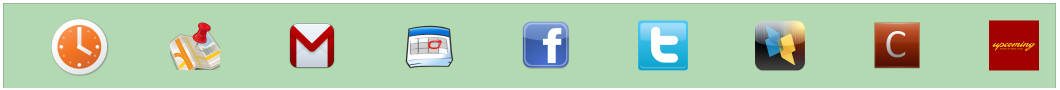
\includegraphics[width=\textwidth]{media/chapter4/stacktrace/sources.png}
\caption{Available Data Sources.}
\label{fig:stacktrace-simple-sources}
\end{minipage}
\end{figure}

\begin{figure}[h]
\centering
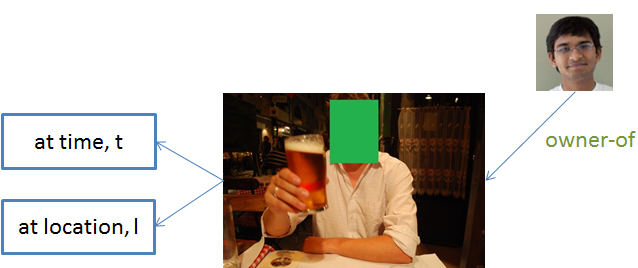
\includegraphics[width=0.75\textwidth]{media/chapter4/stacktrace/init-network.png}
\caption{Context Network built after User Information and EXIF sources are queried and merged.}
\label{fig:exif-network}
\end{figure}

Now, the algorithm traverses the graph to list all the possible queries it can execute on the data integration layer. Given the knowledge that entities participate in events, and events can contain participants, it generates the following queries:

\begin{itemize}
\item Does any data source contain participant information related to the photo capture event?
\item What events is the owner (entity:ArjunSatish) participating at time, t and location, l?
\end{itemize}

The data integration system looks at the different sources and says that none of them store information about photo capture events, and skips executing the first query. But many sources describe events, and store their participants too (Google Calendar, Facebook, Conference Calendar). These query is converted to their native formats (API calls or relational database queries) and results, are sent back to the data integration module. We see that there was a calendar entry returned be the Google Calendar source, as shown in \ref{fig:stacktrace-simple-calendar}. This information is now merged with the existing context graph to produce a context graph similar to that shown in \ref{fig:stacktrace-simple-context-network}.

\begin{figure}[h]
\centering
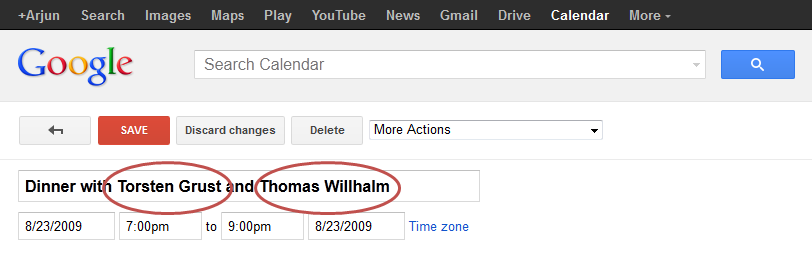
\includegraphics[width=\textwidth]{media/chapter4/stacktrace/calendar.png}
\caption{Calendar Event.}
\label{fig:stacktrace-simple-calendar}
\end{figure}

\begin{figure}[h]
\centering
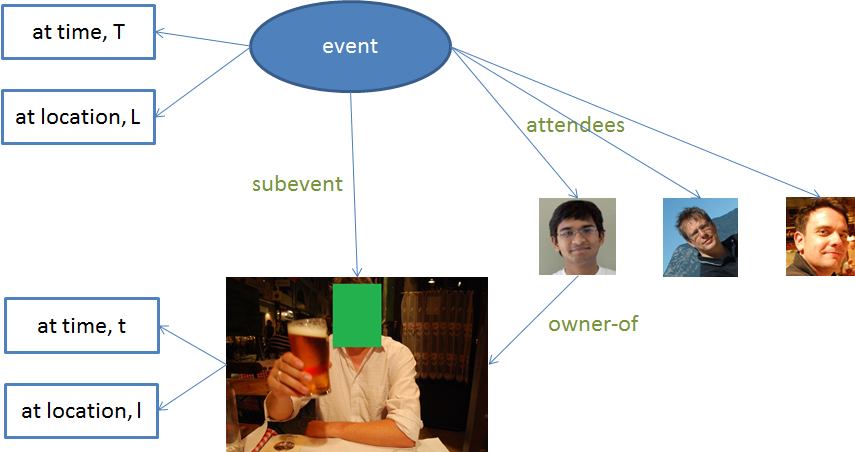
\includegraphics[width=0.75\textwidth]{media/chapter4/stacktrace/context-network-torsten.png}
\caption{Context Network after integrating calendar information.}
\label{fig:stacktrace-simple-context-network}
\end{figure}

Now, we have new entities related to the photo. The face verification algorithm is invoked with the new set of candidates. It must be noted that this verification problem is much easier than trying to verify out of many thousands of candidates. Once the correct entity is identified, the photo is annotated as shown in figure \ref{fig:stacktrace-simple-torsten-tagged}.

\begin{figure}[h]
\centering
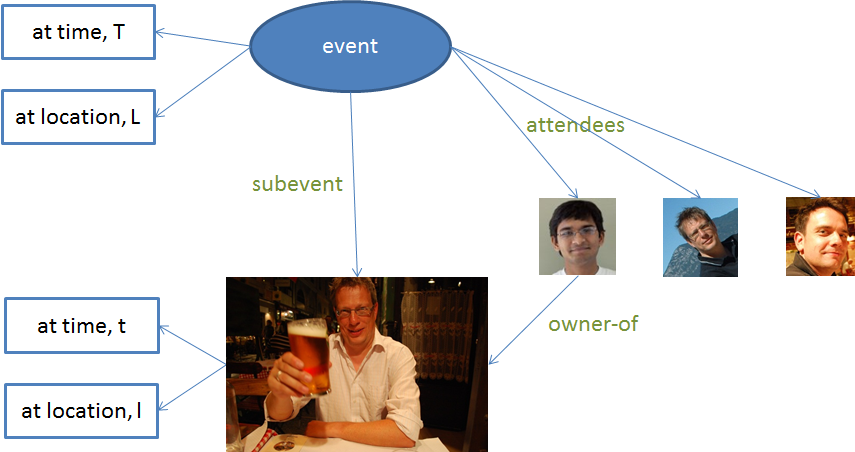
\includegraphics[width=0.9\textwidth]{media/chapter4/stacktrace/torsten-tagged.png}
\caption{The Conceptual Architecture of CueNet.}
\label{fig:stacktrace-simple-torsten-tagged}
\end{figure}

One last look at the source diagram in figure \ref{fig:stacktrace-simple-all} shows which data sources revealed interesting information related to this photo. In this case, EXIF provided some relevant context on when and where the photo was taken. The owner's personal calendar provided information on what event was occurring during the time of photo capture, and who else was involved in it.

\begin{figure}[h]
\centering
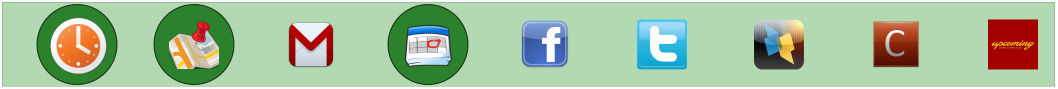
\includegraphics[width=0.75\textwidth]{media/chapter4/stacktrace/time-space-calendar-selected.png}
\caption{Sources which provided relevant context are highlighted by green circles.}
\label{fig:stacktrace-simple-all}
\end{figure}

\subsection{Complex Case}
Now, we will consider a more complex case which requires more than just metadata and personal sources for successful tagging. The photo under consideration is shown in \ref{fig:vldb-hidden}. We will use the same set of data sources, shown again in \ref{fig:vldb-sources}.

\begin{figure}[ht]
\begin{minipage}[b]{0.45\linewidth}
\centering
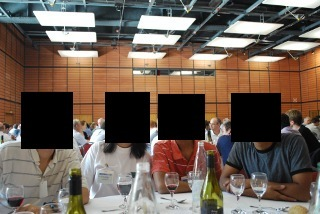
\includegraphics[width=\textwidth]{media/chapter4/stacktrace/vldb-hide-all.jpg}
\caption{Input Photo.}
\label{fig:vldb-hidden}
\end{minipage}
\hspace{0.5cm}
\begin{minipage}[b]{0.45\linewidth}
\centering
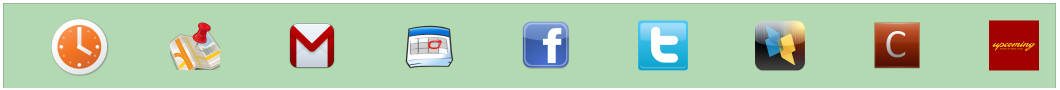
\includegraphics[width=\textwidth]{media/chapter4/stacktrace/sources.png}
\caption{Available Data Sources.}
\label{fig:vldb-sources}
\end{minipage}
\end{figure}

\begin{figure}[h]
\centering
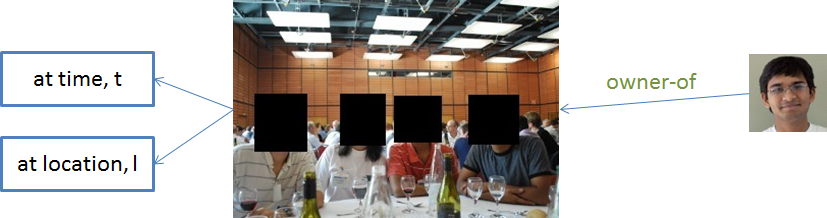
\includegraphics[width=0.9\textwidth]{media/chapter4/stacktrace/vldb-network-1.png}
\caption{Context Network built after User Information and EXIF sources are queried and merged.}
\label{fig:vldb-exif-network}
\end{figure}

Using metadata sources and personal information, we arrive at the context network shown in figure \ref{fig:vldb-exif-network}. The procedure until here is exactly same as that for the previous scenario. Now, given the known state of the world, if we invoke the face verification tools, we discover that the owner is actually present in the photo (figure \ref{fig:vldb-network-2}). In this case, the candidate set contains just one entity, and therefore reduces the complexity of the tagging algorithm.

\begin{figure}[h]
\centering
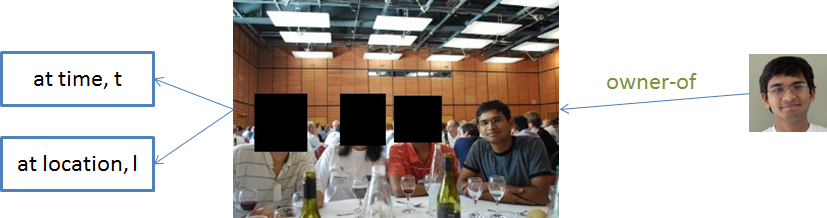
\includegraphics[width=0.9\textwidth]{media/chapter4/stacktrace/vldb-network-2.png}
\caption{Context Network built after User Information and EXIF sources are queried and merged.}
\label{fig:vldb-network-2}
\end{figure}

The next query generated by the system is to discover what the (entity:ArjunSatish) was doing at this time? But, this time we find that the conference calendar holds the answer.

\begin{figure}[h]
\centering
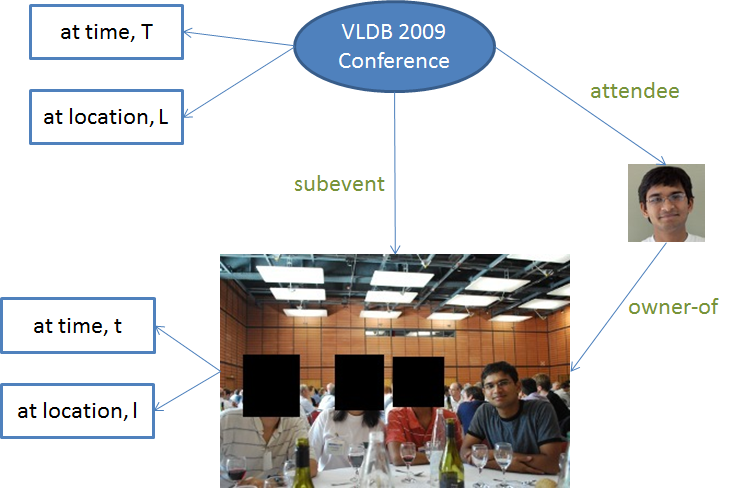
\includegraphics[width=0.75\textwidth]{media/chapter4/stacktrace/vldb-network-3.png}
\end{figure}
\begin{figure}[h]
\centering
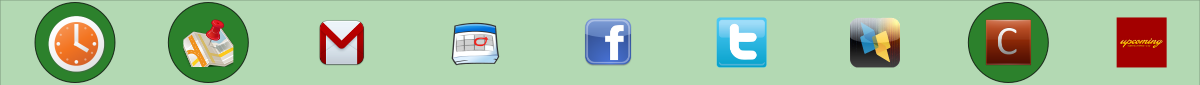
\includegraphics[width=0.9\textwidth]{media/chapter4/stacktrace/vldb-source-1.png}
\caption{Context Network after querying conference sources.}
\label{fig:vldb-network-3}
\end{figure}

At this point, the conference event is known to our knowledge base to have a definite structure, in terms of keynote, session and talk events with lunch/coffee breaks interleaved, and having many attendees. So it immediately queries the conference source to find and merge all of these objects. It discovers that the photo was taken during a break event, and that the conference (VLDB 2009) has many hundreds of participants, as shown in figure \ref{fig:vldb-network-4}.

\begin{figure}[h]
\begin{minipage}[b]{0.5\linewidth}
\centering
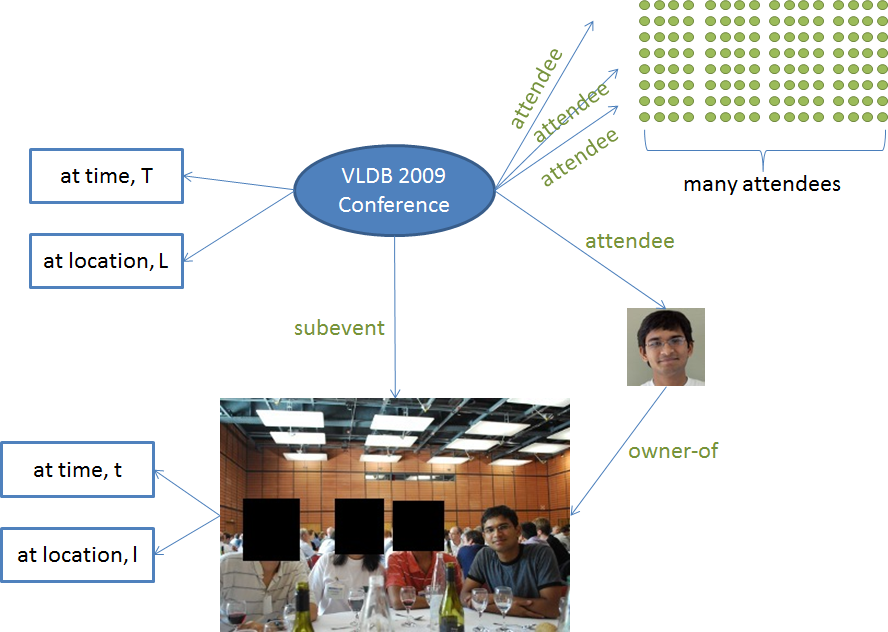
\includegraphics[width=\textwidth]{media/chapter4/stacktrace/vldb-network-4.png}
\caption{Context Network after discovering conference attendees.}
\label{fig:vldb-network-4}
\end{minipage}
\hspace{0.5cm}
\begin{minipage}[b]{0.5\linewidth}
\centering
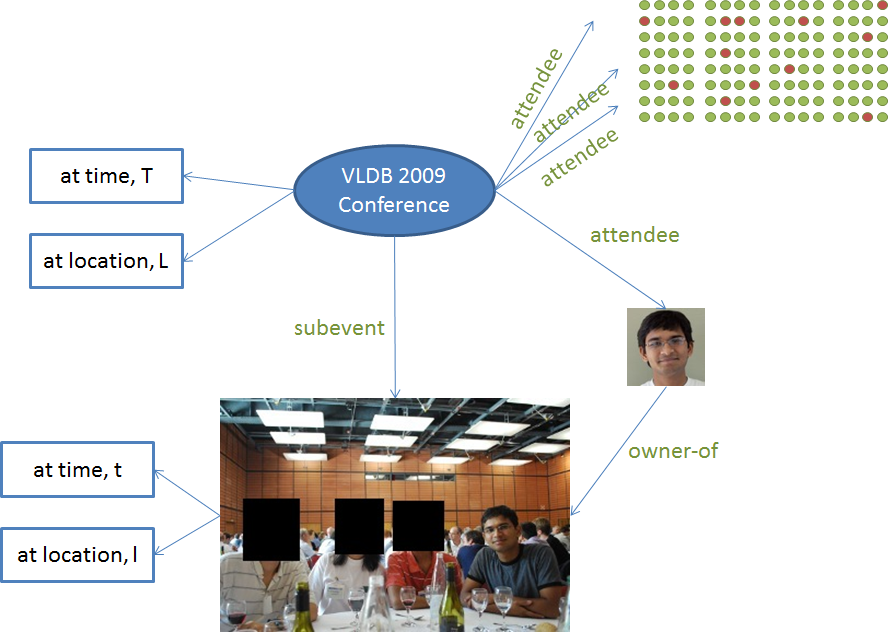
\includegraphics[width=\textwidth]{media/chapter4/stacktrace/vldb-network-5.png}
\caption{Context Network after discovering relations between attendees and owner.}
\label{fig:vldb-network-5}
\end{minipage}
\end{figure}

Figure \ref{fig:vldb-network-4} shows the various attendees discovered by the algorithm from the conference source. But finding 3 candidates from hundreds is an equally challening task. Before invoking the face tagging algorithm, we want to see if we can discover any more relations between the objects in the context network. So the discovery algorithm consults the knowledge base to find that entities can be related through a \textbf{friend-of} relation. So it queries all known sources to find friend relations, and finds that Facebook, Gmail and Twitter are sources which store data containing this relation. Querying it reveals that a few of the entities who were present at the conference were related to the user, and therefore have a bigger chance of appearing in the photo. The face verifier is invoked only with these candidates, for potential true positives. By doing this we tag two more faces in the photo. The context network is shown in the figure \ref{fig:vldb-network-6}.

\begin{figure}[h]
\centering
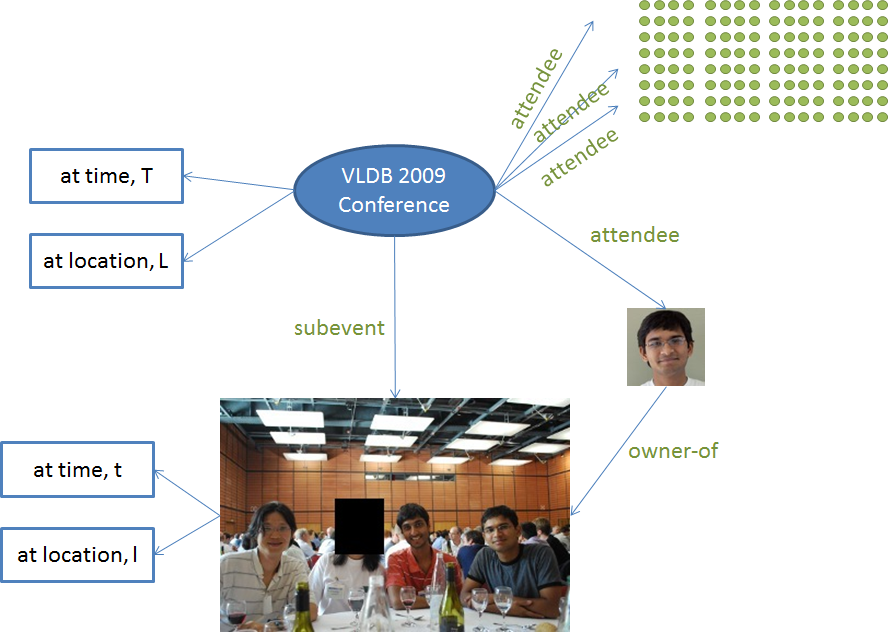
\includegraphics[width=0.75\textwidth]{media/chapter4/stacktrace/vldb-network-6.png}
\caption{Context Network after discovering social relations.}
\label{fig:vldb-network-6}
\end{figure}
\begin{figure}[h]
\centering
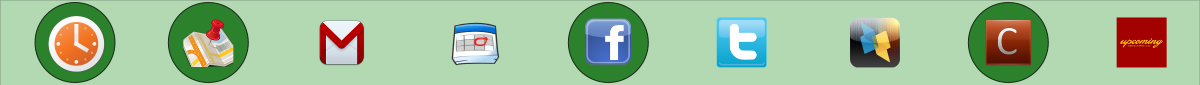
\includegraphics[width=0.9\textwidth]{media/chapter4/stacktrace/vldb-source-2.png}
\caption{Sources used so far.}
\label{fig:vldb-network-3}
\end{figure}

Since we have more candidates tagged in the photo, we can repeat the above procedure to discover more relation between the entites related to the photo and those who are present in the conference. This time results are returned from Gmail, and none from Facebook and Twitter (because these people had sent emails to each other during the conference, but did not connect through Facebook or Twitter). The changes in the context network are shown in \ref{fig:vldb-network-7} and \ref{fig:vldb-network-8}. Figure \ref{fig:vldb-network-3} highlights all sources which returned relevant context for this trace. 

\begin{figure}[h]
\begin{minipage}[b]{0.5\linewidth}
\centering
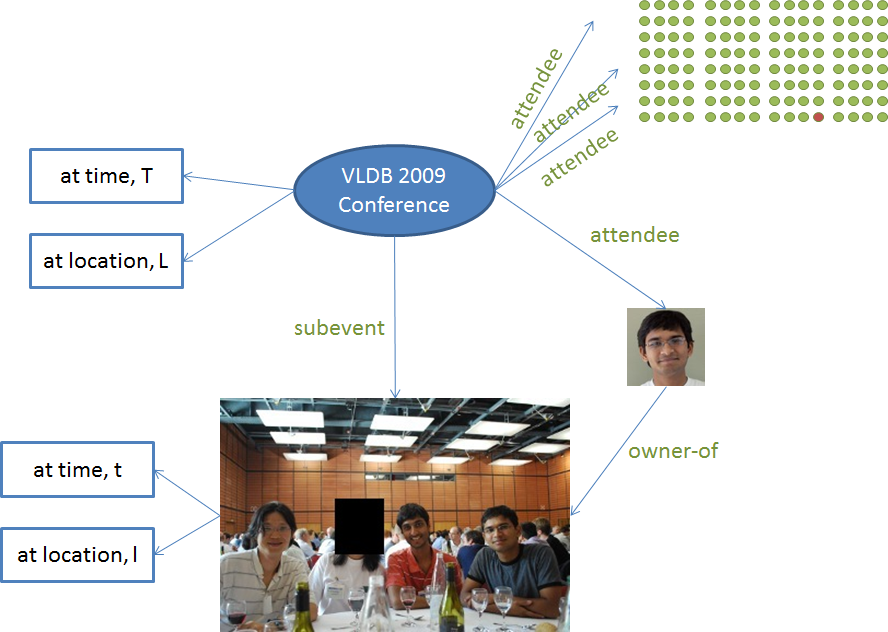
\includegraphics[width=\textwidth]{media/chapter4/stacktrace/vldb-network-7.png}
\caption{Context Network after discovering further social relations.}
\label{fig:vldb-network-7}
\end{minipage}
\hspace{0.5cm}
\begin{minipage}[b]{0.5\linewidth}
\centering
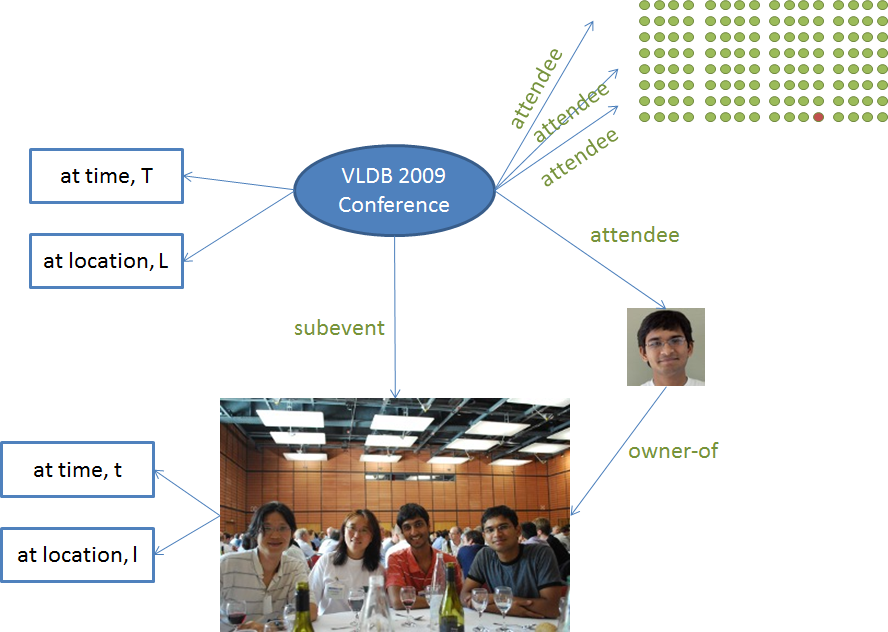
\includegraphics[width=\textwidth]{media/chapter4/stacktrace/vldb-network-8.png}
\caption{Context Network after tagging all faces.}
\label{fig:vldb-network-8}
\end{minipage}
\end{figure}

\begin{figure}[h]
\centering
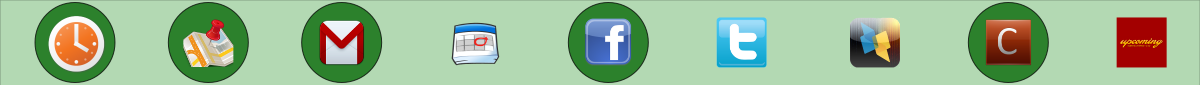
\includegraphics[width=\textwidth]{media/chapter4/stacktrace/vldb-source-3.png}
\caption{Sources used to tag all faces.}
\label{fig:vldb-network-3}
\end{figure}


\section{Event Model}
Our ontologies extend the E* model\cite{gupta2011managing} to specify relationships between events and entities. Specifically, we utilize the relationships ``\textbf{subevent-of}", which specifies event containment. An event $e1$ is a subevent-of of another event $e2$, if $e1$ occurs completely within the spatiotemporal bounds of $e2$. Additionally, we utilize the relations \textbf{occurs-during} and \textbf{occurs-at}, which specify the space and time properties of an event. Also, another important relation between entities and events is the ``\textbf{participant}" property, which allows us to describe which entity is participating in which event. It must be noted that participants of a subevent are also participants of the parent event. A participation relationship between an event and person instance asserts the presence of the person within the spatiotemporal region of the event. We argue that the reverse is also true, i.e., if a participant $P$ is present in $\mathcal{L}_P$ during the time $\mathcal{T}_P$ and an event $E$ occurs within the spatiotemporal region $<\mathcal{L}_E$, $\mathcal{T}_E>$, we say $P$ is a participant of $E$ if the event's spatiotemporal span contained that of the participant.
\begin{equation}
\label{eq:participation-region}
\begin{aligned}
\text{\texttt{participant}(E, P)} \iff (\mathcal{L}_P \sqsubset_L \mathcal{L}_E) \wedge (\mathcal{T}_P \sqsubset_T \mathcal{T}_E)
\end{aligned}
\end{equation}
The symbols $\sqsubset_L$ and $\sqsubset_T$ indicate spatial and temporal containment respectively. Please refer to \cite{gupta2011managing} for more details. In later sections, we refer to the location and time of the event, $\mathcal{L}_E$ and $\mathcal{T}_E$ as $E$.\textbf{occurs-at} and $E.$\textbf{occurs-during} respectively. 

\begin{figure*}[t]
\centering
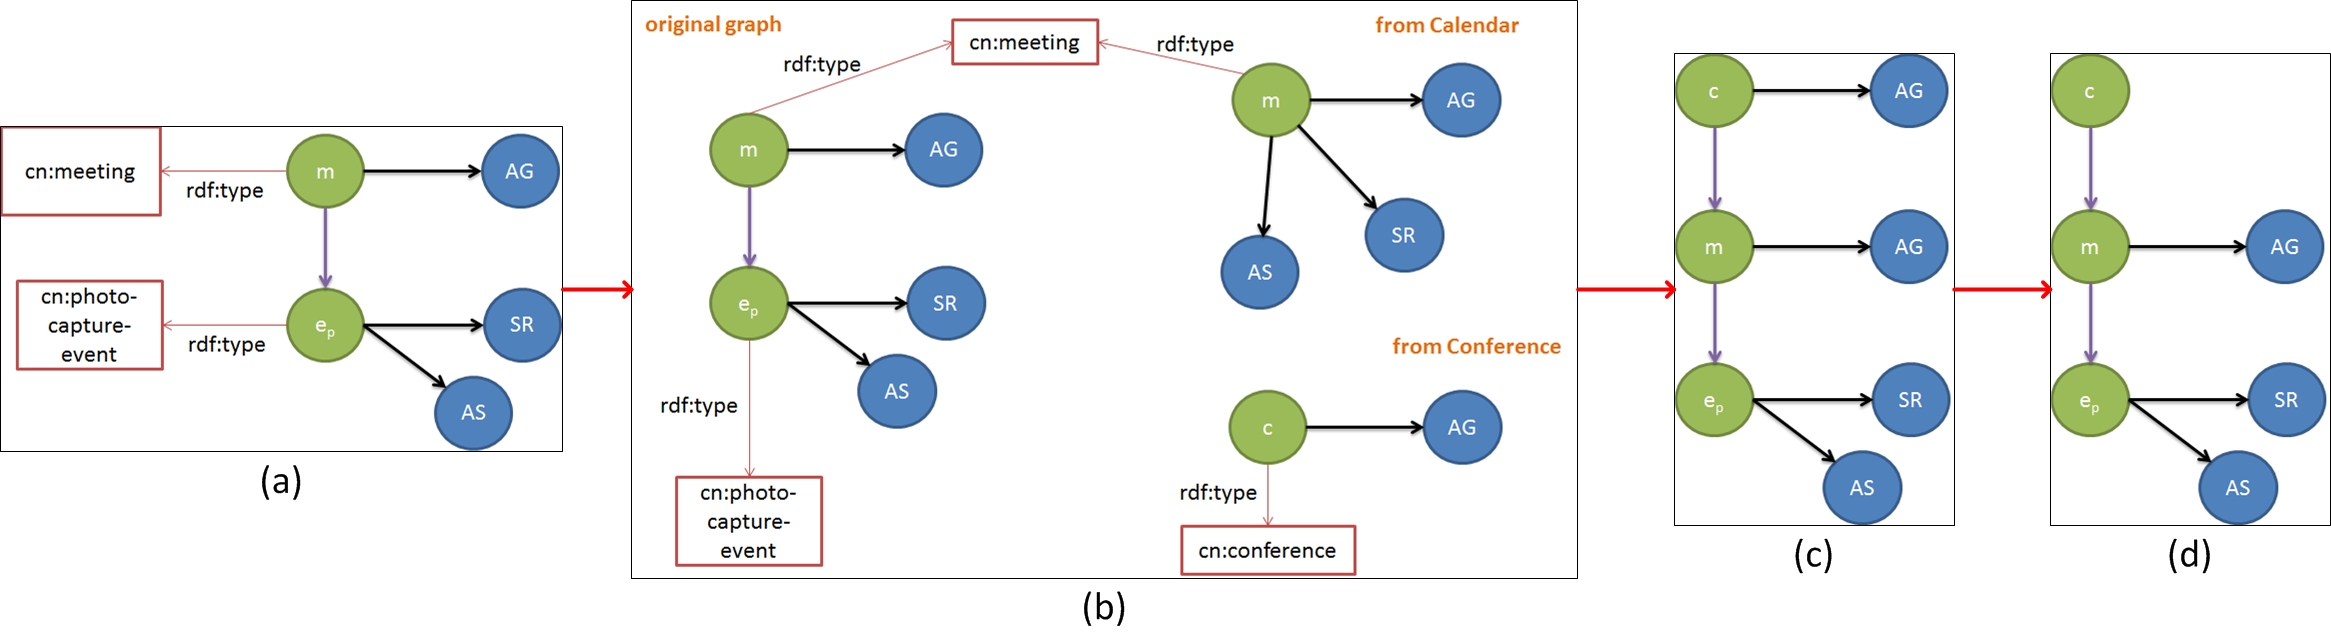
\includegraphics[width=\textwidth]{media/exec/exec-cycle-one-line.png}
\caption{The various stages in an iteration of algorithm \ref{alg:cx-alg}.}
\label{fig:exec-cycle}
\end{figure*}

\section{Data Sources}
\label{sec:data-sources}
The ontology makes available a vocabulary of classes and properties. Using this vocabulary, we can now declaratively specify the schema of each source. With these schema descriptions, CueNet can infer what data source can provide what type of data instances. For example, the framework can distinguish between a source which describes conferences and another which is a social network. We use a LISP like syntax to allow developers of the system to specify these declarations. The example below describes a source containing conference information.

\begin{verbatim}
(:source conferences
   (:attrs url name time location title)
   (:rel conf type-of conference)
   (:rel time type-of time-interval)
   (:rel loc type-of location)
   (:rel attendee type-of person)
   (:rel attendee participant-in conf)
   (:rel conf occurs-at loc)
   (:rel conf occurs-during time)
   (:axioms
      (:map time time)
      (:map loc location)
      (:map conf.title ltitle)
      (:map conf.url url)
      (:map attendee.name name)))
\end{verbatim}

% The above source declaration consists of a s-expression, where the source keyword indicates a unique name for the source. The \texttt{attrs} keyword is used to list the attributes of this source. The \texttt{rel} keyword constructs the instances conf, time, loc, attendee which are of conference, time-interval, location and person class types respectively, and relates them with relations specified in the ontology. Finally, the mapping \texttt{axioms} are used to map nodes in the relationship graph constructed above to attributes of the data source. For example, the first axiom (specified using the map keyword) maps the time node to the time attribute. 

A source declaration comprises of a single nested s-expression. We will refer to the first symbol in each expression as a keyword, and the following symbols as operands. This above declaration uses five keywords (\texttt{source}, \texttt{attrs}, \texttt{rel}, \texttt{axioms}, \texttt{map}).  The \texttt{source} keyword is the root operator, and declares a unique name of the data source. The source mapper can be queried for finding accessors using this name. The \texttt{attrs} keyword is used to list the attributes of this source. Currently we assume a tuple based representation, and each operand in the attrs expression maps to an element in the tuple. The \texttt{rel} keyword allows construction of a relationship graph where the nodes are instances of ontology concepts. And edges are the relationships described by this particular source. In the above example, we construct individuals \textit{conf}, \textit{time}, \textit{loc} and \textit{attendee} who are instances of the \textit{conference}, \textbf{time-interval}, \textbf{location} and \textbf{person} class respectively. We further say that attendee is a \textbf{\textit{participant of}} the conference, which \textbf{\textit{occurs-at}} location loc and \textbf{\textit{occurs-during}} the interval time. Finally, the \texttt{mapping axioms} are used to map nodes in the relationship graph to attributes of the data source. For example, the first axiom (specified using the map keyword) maps the time node to the time attribute. The third map expression creates a literal called title, and associates it to the conference node, whose value comes from the ltitle attribute of the conference data source.

Formally, we represent the given ontology as $O$. The various classes and properties in $O$ are represented by $C^O$ and $P^O$ respectively. Since our upper ontology consists of DOLCE and E*, we assume the inclusion of the classes \texttt{Endurant}, \texttt{Perdurant}, \texttt{Event} and \texttt{Person} in $C^O$. Each source $S$ consists of three parts, a relation graph $G^S(V^S, E^S)$ where the nodes $V^S \in C^O$, specify the various ``things'' described by the source. The edges $E^S \in P^O$ specify the relations among the nodes. Any graph retrieved from such a source is an instance of the relation graph, $G^S$. Further, the tuple $A^S_T$ consists of the attributes of the data source. Finally, the mapping $M^S: \{G^S \rightarrow A^S_T\}$ specifies how to map different nodes in the relation graph to the different attributes of the native data source.

\section{Conditions for Discovery}
CueNet is entirely based on reasoning in the event and entity (i.e., person) domain, and the relationships between them. These relationships include participation (event-entity relation), social relations (entity-entity relation) and subevent relation (event-event). For the sake of simplicity, we restrict our discussions to events whose spatiotemporal spans either completely overlap or do not intersect at all. We do not consider events which partially overlap. In order to develop the necessary conditions for context discovery, we consider the following two axioms:

\textbf{Entity Existence Axiom}: Entities can be present in one place at a time only. The entity cannot exist outside a spatiotemporal boundary containing it.

\textbf{Participation Semantics Axiom}: If an entity is participating in two events at the same time, then one is the subevent of the other. 

% Before we provide an overview of the discovery algorithm, we must make a note of set of conditions required for its correct execution. 

Given, the ontology $O$, we can construct event instance graph $G^I(V^I, E^I)$, whose nodes are instances of classes in $C^O$ and edges are instances of the properties in $P^O$. The context discovery algorithm relies on the notion that given an instance graph, \textit{queries} to the different sources can be automatically constructed. A query is a set of predicates, with one or more unknown variables. For the instance graph $G^I (V^I, E^I)$, we construct a query $Q(D, U)$ where $D$ is a set of predicates, and $U$ is a set of unknown variables.

\textbf{Query Construction Condition:} Given an instance graph $G^I (V^I, E^I)$ and ontology $O(C^O, P^O)$, a query $Q(D, U)$ can be constructed, such that $D$ is a set of predicates which represent a subset of relationships specified in $G^I$. In other words, $D$ is a subgraph induced by $G^I$. $U$ is a class, which has a relationship $r \in P^O$, with a node $n \in D$. Essentially, the ontology must prescribe a relation between some node $n$ through the relationship $r$. In our case, the relation $r$ will be either a \textbf{participant} or \textbf{subevent} relation. If the relationship with the instances does not violate any object property assertions specified in the ontology, we can create the query $Q(D, U)$.

\textbf{Identity Condition:} Given an instance graph $G^I(V^I, E^I)$, and a result graph $G^R(V^R, E^R)$ obtained from querying a source, we can merge two events only if they are identical. Two nodes $v^I_i \in V^I$ and $v^R_r \in V^R$ are identical if they meet the following two conditions \textbf{(i)} Both $v^I_i$ and $v^R_r$ are of the same class type, and \textbf{(ii)} Both $v^I_i$ and $v^R_r$ have exactly overlapping spatiotemporal spans, indicated by the $=_L$ and $=_T$. Mathematically, we write: 
\begin{equation}
\label{eq:identity}
\begin{aligned}
v^I_i = v^R_r \iff (v^I_i.\text{\textbf{type-of}} = v^R_r.\text{\textbf{type-of}}) \wedge \\ 
(v^I_i.\text{\textbf{occurs-at}} =_L v^R_r.\text{\textbf{occurs-at}}) \wedge \\
(v^I_i.\text{\textbf{occurs-during}} =_T v^R_r.\text{\textbf{occurs-during}})
\end{aligned}
\end{equation}
\textbf{Subevent Condition:} Given an instance graph $G^I(V^I, E^I)$, and a result graph $G^R(V^R, E^R)$ obtained from querying a source, we can construct a subevent edge between two nodes $v^I_i \in V^I$ and $v^R_r \in V^R$, if one is spatiotemporally contained within the other, and has at least one common \texttt{Endurant}.
\begin{equation}
\label{eq:sube-st-containment}
\begin{aligned}
   v^I_i \sqsubset_L v^R_r,\\
   v^I_i \sqsubset_T v^R_r
\end{aligned}
\end{equation}
\begin{equation}
\label{eq:sube-entity-containment}
\begin{aligned}
   v^I_i.\text{\textbf{Endurants}} \cap v^R_r.\text{\textbf{Endurants}} \neq \{\phi\}\\
\end{aligned}
\end{equation}
Here $v^I_i.$\textbf{Endurants} is defined as a set $\{w | w \in V^I_i \wedge w.$type-of$ = $Endurant$\}$. If equation \eqref{eq:sube-entity-containment} does not hold, we say that $v^I_i$ and $v^R_r$ co-occur.

\textbf{Merging Event Graphs}: Given the above conditions, we can now describe an important building block for the context discovery algorithm: the steps needed to merge two event graphs. An example for this is shown in figure \ref{fig:exec-cycle}(b-d). Given the event graph consisting of the photo capture event on the left of (b) and a meeting event $m$ and conference event $c$, containing their respective participants. In this example, the meeting event graph, $m$ is semantically equivalent to the original graph. But the conference event, $c$ is telling that the person $AG$ is also participating in a conference at the time the photo was taken. The result of merging is shown in (d). An event graph merge consists of two steps. The first is a \texttt{subevent hierarchy join}, and the second is a \texttt{prune-up} step. 

Given an original graph, $O_m$, and a new graph $N_m$, the join function works as follows: All nodes in $N_m$ are checked against all nodes in $O_m$ to find identical counterparts. For entities, the identity is verified through an identifier, and for events, equation \eqref{eq:identity} is used. Because of the entity existence and participation semantics axioms, all events which contain a common participant are connected to their respective super event using the subevent relation (equations \eqref{eq:sube-st-containment} and \eqref{eq:sube-entity-containment} must be satisfied by the events). Also, if two events have no common participant, then they can be still be related with the subevent edge, if the event model says it is possible. For example, if in a conference event model, keynotes, lunches and banquets are declared as known subevents of an event. Then every keynote event, or banquet event to be merged into an event graph is made a subevent of the conference event, if the equation \eqref{eq:sube-st-containment} holds between the respective events. 

It must be noted that node $AG$ occurs twice in graph (c). In order to correct this, we use the participation semantics axiom. We traverse the final event graph from the leaves to the root events, and remove every person node if it appears in a subevent. This is the \texttt{prune-up} step. Using these formalisms, we now look at the working of the context discovery algorithm. 

\restylealgo{ruled}
\SetAlgoSkip{}
\begin{algorithm}[h]
\dontprintsemicolon 
\KwData{A photograph H, with a set of detected faces F. Voting threshold, T. The owner O of the photo.}
\KwResult{For each face f $\in$ F, a set of atmost $k$ person tags.}
\Begin{
  
  $ $\;
  function discover(): \{ \;
  \Indp while (\texttt{DQ} is not empty): \{ \;
  \Indp \texttt{node} = \texttt{DQ}.deque() \;
  \texttt{results} = query (\texttt{node}) \;
  \texttt{E} $\leftarrow$ merge (\texttt{E}, \texttt{results}) \;
  if (termination\_check()): \;
  \Indp \textbf{return} prepare\_results(); \;
  \Indm
  \Indm
  \} \;
  reconstruct \texttt{DQ} $\leftarrow$ \texttt{E} \;
  discover() \;
  \Indm
  \}\;
  
  $ $\;
  
  function merge(\texttt{O}, \texttt{N}): \{ \;
    \Indp 
    remove\_duplicates() \;
    \texttt{M} $\leftarrow$ subevent\_hierarchy\_join(\texttt{O}, \texttt{N}) \;
    prune\_up(\texttt{M}) \;
    if (less than \texttt{T} new candidates were discovered): \; {
    \Indp
  	    push\_down(\texttt{M}) \;
  	\Indm
    } else: \; 
    \Indp
	    vote\_and\_verify(\texttt{M}) \;
  	\Indm
 	return \texttt{M}; \;
  \Indm
  \} 
  
  $ $ \;
  \texttt{E} $\leftarrow$ construct event graph with \texttt{H} and \texttt{O} \;
  construct discoverable nodes queue, \texttt{DQ} $\leftarrow$ \texttt{E} \;
  \textbf{return} discover() \;
  
}
\caption{The Context Discovery Algorithm}
\label{alg:cx-alg}
\end{algorithm}

\subsection{Context Discovery Algorithm}
\label{sec:discovery-algorithm}
Algorithm \ref{alg:cx-alg} below outlines the tail recursive discovery algorithm. The input to the algorithm is a photo (with EXIF tags) and an associated owner (the user). It must be noted that by seeding the graph with owner information, we bias the discovery towards his/her personal information. An event instance graph is created where each photo is modeled as a photo capture event. Each event and entity is a node in the instance graph. Each event is associated with time and space attributes. All relationships are edges in this graph. All EXIF tags are literals, related to the photo with data property edges. Figure \ref{fig:exec-cycle} graphically shows the main stages in a single iteration of the algorithm.

The event graph is traversed to produce a queue of entity and event nodes, which we shall refer to as DQ (discovery queue). The algorithm consists of two primary functions: \textbf{discover} and \textbf{merge}. The discover function is tail recursive, invoking itself until a termination condition is reached (when at most $k$ tags are obtained for all faces or no new data is obtained from all data sources for all generated queries). The behavior of the query function depends on the type of the node. If the node is an event instance, the function consults the ontology to find any known sub-events, and queries data sources to find all these subevents, its properties and participants of the input event node. On the other hand, if it is an entity instance, the function issues a query to find all the events it is participating in. 

Results from data source wrappers are returned in the form of event graphs. These event graphs are merged into the original event graph by taking the following steps. First, it identifies \textbf{duplicate} events using the conditions mentioned above. Second, it identifies subevent hierarchies using the graph merge conditions described above, and performs a \textbf{subevent hierarchy join}. Third, the function \textbf{prune-up} removes entities from an event when its subevent also lists it as a participant node. Fourth, \textbf{push-down} is the face verification step if the number of entities in the parents of the photo-capture events is small (less than $T$). Push down will try to verify if any of the newly discovered entities are present in the photo and if they are (if the tagging confidence is higher than the given threshold), the entities are removed from the super event, and linked to the photo capture event as its participant. On the other hand, if this number is larger than T, the algorithm initiates the \textbf{vote-and-verify} method, which ranks all the candidates based on social relationships with people already identified in the photo. For example, if a candidate is related to two persons present in the photo through some social networks, then its score is 2. Ranking is done by simply sorting the candidate list by descending order of score. The face verification runs only on the top ranked $T$ candidates. If there are still untagged faces after the termination of the algorithm, we vote over all the remaining people, and return the ranked list for each untagged face.

Figure \ref{fig:exec-cycle} shows the various stages in the algorithm graphically. (a) shows an example event graph describing a photo taken at a meeting. The meeting consists of three participants AG, SR and AS. The photo contains SR and AS. (b) shows two events returned from the data sources. One is a meeting event which is semantically identical to the input. The other is a conference event with AG. (c) shows the result of merging these graphs. (d) The \texttt{prune-up} function removes the duplicate reference to AG. \underline{A live visualization of these steps for different photos can be found at \href{http://cuenet.site44.com/}{http://cuenet.site44.com}}.

\section{Merging Context Networks}

\section{Implementation}

\begin{figure}[t]
\centering
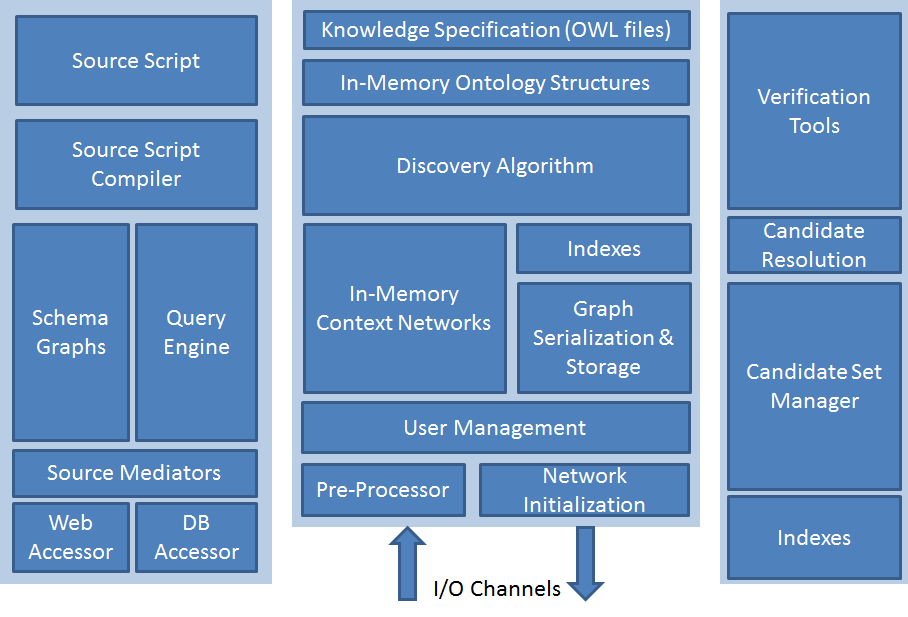
\includegraphics[width=\textwidth]{media/chapter4/detailed-concept-arch.png}
\caption{Sources used to tag all faces.}
\label{fig:d-concept-arch}
\end{figure}

In this section, we will look at the current implementation of the CueNet framework. Figure \ref{fig:d-concept-arch} shows a detailed conceptual architecture of the framework. It consists of three verticals: the data integration modules on the left side, the discovery algorithm and its supporting components in the middle, and the candidate management and face verification tools on the right side. Let's look at them one by one. The data integration module is configured using a source script. This script contains the schema declarations of the various sources, and specifications of how the objects in these sources are related to the objects in the ontology. The complete script listing is provided in Appendix A. We use JavaCC to construct the compiler for this script. The schema and the relations are stored as graphs which can be queried by other modules. Any discover query to be executed on the multitude of sources is checked upon each graph to see if can respond to the type of query. For example, exclude social networks when queries are requesting event information. Each source requires mediator code to align its content with that of the tuples requested in the query engine. This approach is more reminiscent of GAV designs in data integration vocabulary. We chose this because of simpler query processing designs, and the fact that although we required to plug-in and out sources easily, these sources themselves changed very rarely. At the bottom of the data integration stack, we find some common utilities to make HTTP requests and DB query requests, which are used by the source mediators.

Now, lets look at the various components making up the discovery algorithm. Our knowledge base is specified using OWL ontologies. This is parsed using the open source Jena library, and the objects and relations specified are loaded into in memory DAGs. When a tag discovery request is made by a user, the discovery algorithm is initialized with a photo-capture-event, EXIF information is extracted through perl-based exiftool, and the seed context network is constructed and provided to the discovery algorithm. The algorithm initiates the discover and merge operations using the query engine, and the candidate manager. As new relations are discovered, the related entities are then checked for their presence in the photo using verification tools. We used face.com until its termination in mid-2012, after which we use the system based on \cite{nk_attribute_classifiers} until early 2013, after which we resorted to manual verification upon the top ranked candidates.

When a tag request is initiated, a message is passed to the candidate manager, which scans the user's database to create a list of all entities. This is done by invoking scan queries on all data sources through the query engine. Each data sources has a different representation for the same entity. The job of the candidate manager is to aggregate entities by using cues based on their common names or emails, pass them to an entity resolver (if the data is stored on a web-page), and if needed ask a user to correct any mistakes it made in this process. Ultimately, at the end of its processing, we obtain a list of candidates, each which holds identifiers which are local to each data source. When a context network is created by the source mediator, it looks up the candidate reference through the candidate manager before emitting the network back to the discover algorithm. This step makes the nature of data sources oblivious to the discovery algorithm.

\begin{figure}[h]
\centering
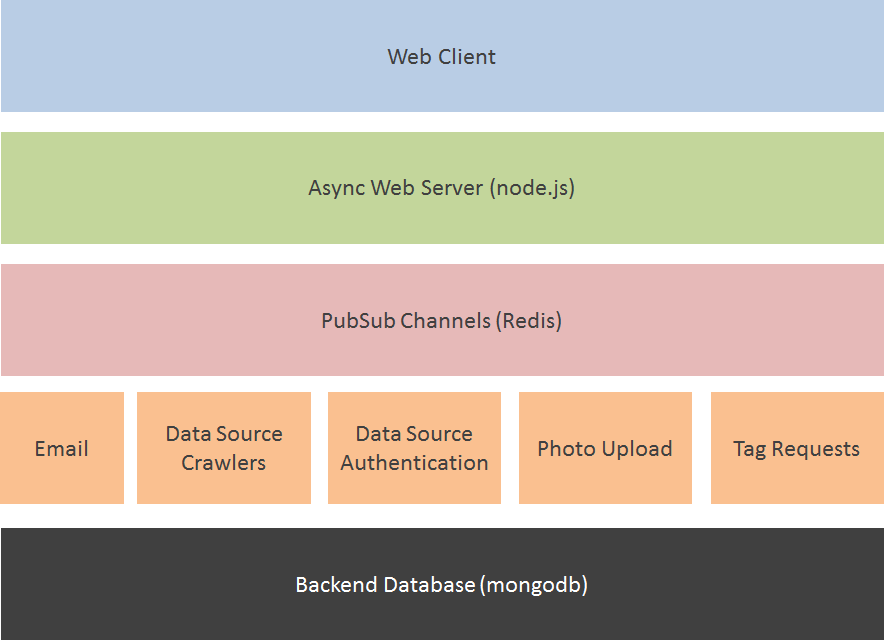
\includegraphics[width=\textwidth]{media/chapter4/web-stack.png}
\caption{Web stack for data aggregation.}
\label{fig:web-stack}
\end{figure}

The web interface to the system is shown in figure \ref{fig:web-stack}. This stack is essential in aggregating data from various sources, and is instrumental in dealing with their intricacies related to authentication, API requests and data formatting. Sources like Facebook and Google have rigid authentication mechanisms which need to be bypassed before any personal data can be accessed. Obtaining user permission needs to be done via a web client for Google APIs, whereas Facebook requires a valid session key from a user. These small details prompted us to implement the data aggregations using Javascript APIs which are served using an asynchronous web server based on node.js. The asynchronous nature of the server allows to implement client which execute a large number of HTTP callbacks without worrying about multi-threading issues -- a design decision which is becoming increasingly popular for web architecture. Once the data has been aggregated at the client, it is passed back to the server which pushes it to specific process which can deal with processing it. For example, email information is sent to an independent Python process which initiates the IMAP protocol on the user's message server to aggregate emails. The Facebook events, social network, photo tag and Google calendar information is sent to a script which loads them into appropriate mongodb collections. Unstructured data like conference webpages are sent to a process which initiates the SNER over them to aggregate entities. These entities are stored in appropriate collections. The server communicates through these processes using REDIS, an in memory cache/database which supports PubSub channels. Multiple channels are created, one for each \textit{type} of data source. Any process can listen to it, obtain the data, process it of its own accord.

\begin{figure}[h]
\centering
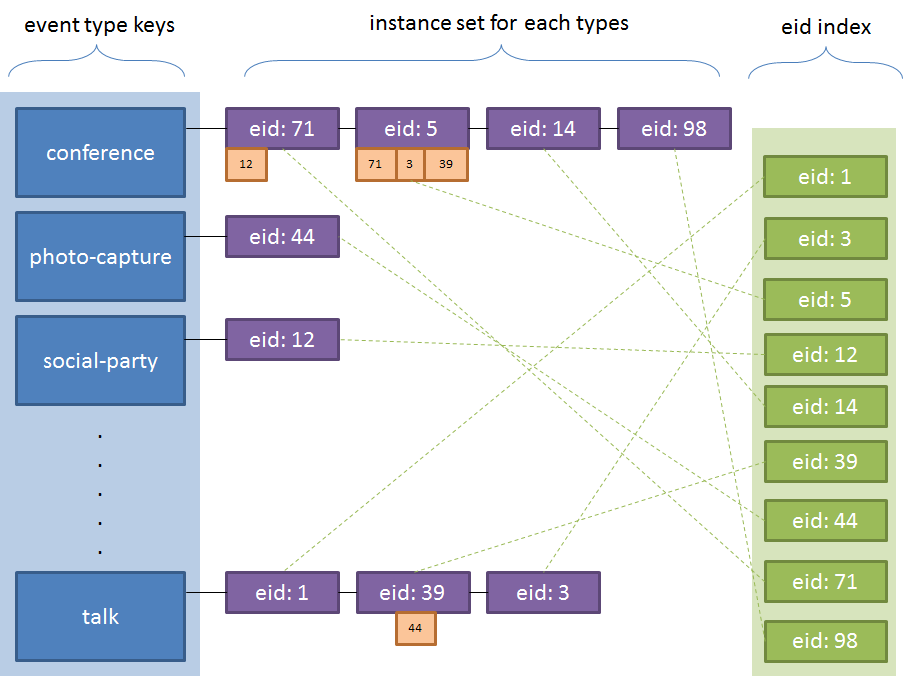
\includegraphics[width=\textwidth]{media/chapter4/adj-list.png}
\caption{The data structure for maintaining Context Network.}
\label{fig:adj-list}
\end{figure}

Lastly, we will describe the data structures used to hold context networks. A context network is a directed graph containing event, and entity nodes, and their relationships. Any standard directed graph implementation can be used to hold this, but given the operations we perform on these network, some additional properties can be exploited to achieve faster merges. One operation we need often is to eliminate merging networks which provide no new information. For this purpose we modify the adjacency list structure to look like the one in figure \ref{fig:adj-list}. A traditional adjacency list holds a hash-table for nodes, and each node is associated with a linked list or another hash-table for the nodes which it connects to. Since IDs don't hold any special meaning between context networks, we cannot rely only on them to distinguish between events in separate context networks. Event identity is established based on type, spatial and temporal information. For this purpose, our primary hash-table contains the \textbf{types} of events present in the network. In the example figure \ref{fig:adj-list}, we see the events of types \texttt{conference}, \texttt{photo-capture}, \texttt{social-party} and \texttt{talk} are contained in the network. For each event type, we associate a list of instances to it. This is implemented currently using a HashSet. Each instance in the context network is identified by a unique instance Id. This architecture allows us to quickly compare new events to existing ones and eliminate duplicates. 

Edge relations are maintained by a list of (instance-id, edge-type) pairs. Thus traversing a network implies starting from a root node, looking up the instance Ids of the outgoing edges by scanning the HashSet, looking the outgoing nodes in the adjacency list, and repeating the process. In order to avoid multiple lookups, we maintain an additional hash-table over instance IDs. Given an instance ID, this table allows fast lookups to avoid time spent in scanning very large sets which are created when there are many instances of the same type of events.

This architecture suffices because we discover context for a single photo at a time. In the case where an application needs to discover context for many events, we use a separate network for each atomic event under consideration, and assume that the context for one event is independent of the other. Thus, a merge operation reduces to finding the existing context network it can be merged with, and performing the merge only with one such network. This assumption will not be true if the events are spatio-temporally very close to each other. Here, information about one event will affect events in the other. This is beyond the scope of this dissertation. We also use a R-Tree built using the Java Spatial Index library to index the time intervals of the events of the various context networks (which do not have any super-events themselves), to reduce the search during the merge step. This increases the overall efficiency of discovery algorithm.